\section{Convolutional Neural Network}
\subsection{Vectorized convolution by Im2col and col2im}
The convolution operation can be implemented by many loops because the kernel will travel over the image. In terms of complexity, this is the easiest way to program but regard to timing, this idea is not efficient since it can only perform a convolution calculation sequentially. Now, with the highly support of hardward (explicitly GPU) that allows us to accelerate even more with parallel computation. In this part, we would like to break down 2 approaches in order to analyse their advantages and downsides.\par

In Im2col, we will trade off some memory for faster computation by trasforming the 3 -channels image to a matrix form in which the convolution operation can be performed more efficiently. We list out 3 stages to implement the efficient way to do vectorized convlution:
\begin{enumerate}
    \item Im2Col for input image and reshape the kernel: transform image and kernel to column form
    \item Do the matrix multiplication between Im2Col output and reshaped kernel
    \item Reshape the output of matrix multiplication to the form of convolution output.
\end{enumerate}
In particular, for step 1, the intensity values of images are within the sliding window will be flatten to a column, then the matrix will consist of many transformed columns like this, covering all the sliding position of the kernel scans through the images, check out figure~\ref{fig:im2col}. Moreover, in the case the image is colored (presumably 3 channels RGB), the output is the concatenated matrix by Im2col output with respect to 3 channels. Obviously, in order to make matrix multiplication feasible, the kernel need to be reshaped to row vector form as well (refer figure~\ref{fig:reshaped_kernels},\ref{fig:reshaped_kernels_3_channels}).\par

Then the $2^{nd}$ step is to do matrix multiplication between Im2Col output and reshaped kernels. Thus the result of 3-channels vectors multiply with 3-channels reshaped kernels rows is a single numeric value (figure~\ref{fig:matrix_multiplication}). Once the we found the matrix output of step 2, we need to convert this matrix into the form of convolution operation's result. For example, regardless padding option and set stride as 1, the image size $7\times7\times 3$ convolves with $3\times 3 \times N$ kernels will produce $5\times 5 \times N$ matrix (note: the number N is usually refered to the number of filter/the depth of feature map respectively for kernel/feature map case). So the output of matrix multiplication for vectorized convolution has the size $5\times(5*N)$ will be reshaped back to form $5\times 5 \times N$ (figure~\ref{fig:matrix_multiplication})


\begin{figure}[H]
    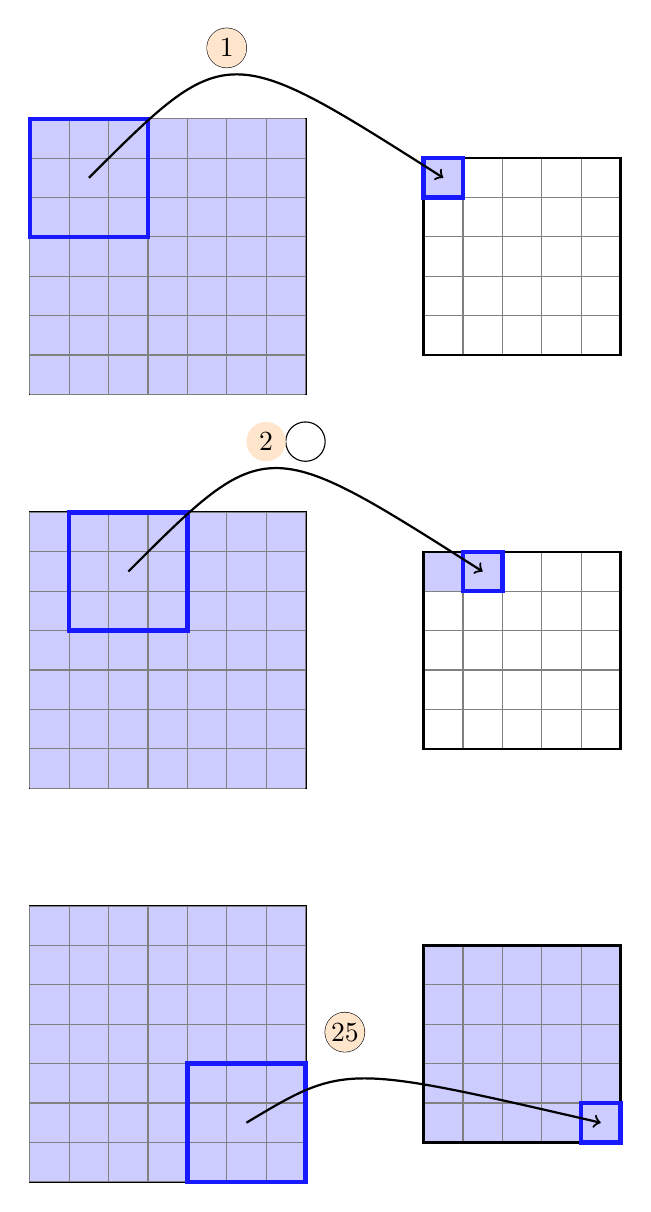
\begin{tikzpicture}
        \begin{scope}[scale=0.5]
            % Draw input convolution
            % Draw the outer rectangle border
            \draw[thick] (0,0) rectangle (7,7);
            
            % Fill the entire 7x7 grid area with a light blue color
            \fill[blue!20] (0,0) rectangle (7,7);
       
            % Draw the boundary of each grid
            \draw[step=1cm, gray, thin] (0,0) grid (7,7);

            % Draw kernel convolution
            % Draw the outer rectangle border
            \draw[ultra thick,blue!90] (0,4) rectangle (3,7);

            % Draw output of convolution
            % Fill the entire 7x7 grid area with a light blue color
            \fill[blue!20] (10,5) rectangle (11,6);
       
            % Draw the boundary of each grid
            \draw[step=1cm, gray, thin] (10,1) grid (15,6);
            
            % Draw the outer rectangle border
            \draw[thick] (10,1) rectangle (15,6);
            \draw[ultra thick,blue!90] (10,5) rectangle (11,6);

            % arrow from kernel to output
            \draw[->,thick] (1.5,5.5) .. controls (5,9) .. (10.5,5.5);
            

            \draw[thin] (5,8.8) circle (0.5cm);
            \fill[orange!20] (5,8.8) circle (0.5cm);
            \node at (5,8.8) {1};
        \end{scope}


        \begin{scope}[scale=0.5,yshift=-10cm]
            % Draw input convolution
            % Draw the outer rectangle border
            \draw[thick] (0,0) rectangle (7,7);
            
            % Fill the entire 7x7 grid area with a light blue color
            \fill[blue!20] (0,0) rectangle (7,7);
       
            % Draw the boundary of each grid
            \draw[step=1cm, gray, thin] (0,0) grid (7,7);

            % Draw kernel convolution
            % Draw the outer rectangle border
            \draw[ultra thick,blue!90] (1,4) rectangle (4,7);
           

            % Draw output of convolution
            % Fill the entire 7x7 grid area with a light blue color
            \fill[blue!20] (10,5) rectangle (12,6);
       
            % Draw the boundary of each grid
            \draw[step=1cm, gray, thin] (10,1) grid (15,6);
            
            % Draw the outer rectangle border
            \draw[thick] (10,1) rectangle (15,6);
            \draw[ultra thick,blue!90] (11,5) rectangle (12,6);

            % arrow from kernel to output
            \draw[->,thick] (2.5,5.5) .. controls (6,9) .. (11.5,5.5);
            
            \draw[thin] (7,8.8) circle (0.5cm);
            \fill[orange!20] (6,8.8) circle (0.5cm);
            \node at (6,8.8) {2};
        \end{scope}


        \begin{scope}[scale=0.5,yshift=-20cm]
            % Draw input convolution
            % Draw the outer rectangle border
            \draw[thick] (0,0) rectangle (7,7);
            
            % Fill the entire 7x7 grid area with a light blue color
            \fill[blue!20] (0,0) rectangle (7,7);
       
            % Draw the boundary of each grid
            \draw[step=1cm, gray, thin] (0,0) grid (7,7);

            % Draw kernel convolution
            % Draw the outer rectangle border
            \draw[ultra thick,blue!90] (4,0) rectangle (7,3);
           

            % Draw output of convolution
            % Fill the entire 7x7 grid area with a light blue color
            \fill[blue!20] (10,1) rectangle (15,6);
       
            % Draw the boundary of each grid
            \draw[step=1cm, gray, thin] (10,1) grid (15,6);
            
            % Draw the outer rectangle border
            \draw[thick] (10,1) rectangle (15,6);
            \draw[ultra thick,blue!90] (14,1) rectangle (15,2);

            % arrow from kernel to output
            \draw[->,thick] (5.5,1.5) .. controls (8,3) .. (14.5,1.5);
            
            \draw[thin] (8,3.8) circle (0.5cm);
            \fill[orange!20] (8,3.8) circle (0.5cm);
            \node at (8,3.8) {25};
        \end{scope}

    \end{tikzpicture}
    \centering
    \caption{Convolution operation between $7\times7$ input and $3\times3$ kernel filter with $stride=1$. If we use a loop then each iteration we slide over a $3\times3$ subgrid of input, we have to do9 multiplications and 8 addition. The number operations we have to do is $9\times8\times25=1800$ operations for 1 convolution. Remind that with this looping implementation, we can only do $9\times8=72$ operations sequentially.}
\end{figure}



\begin{figure}[H]
    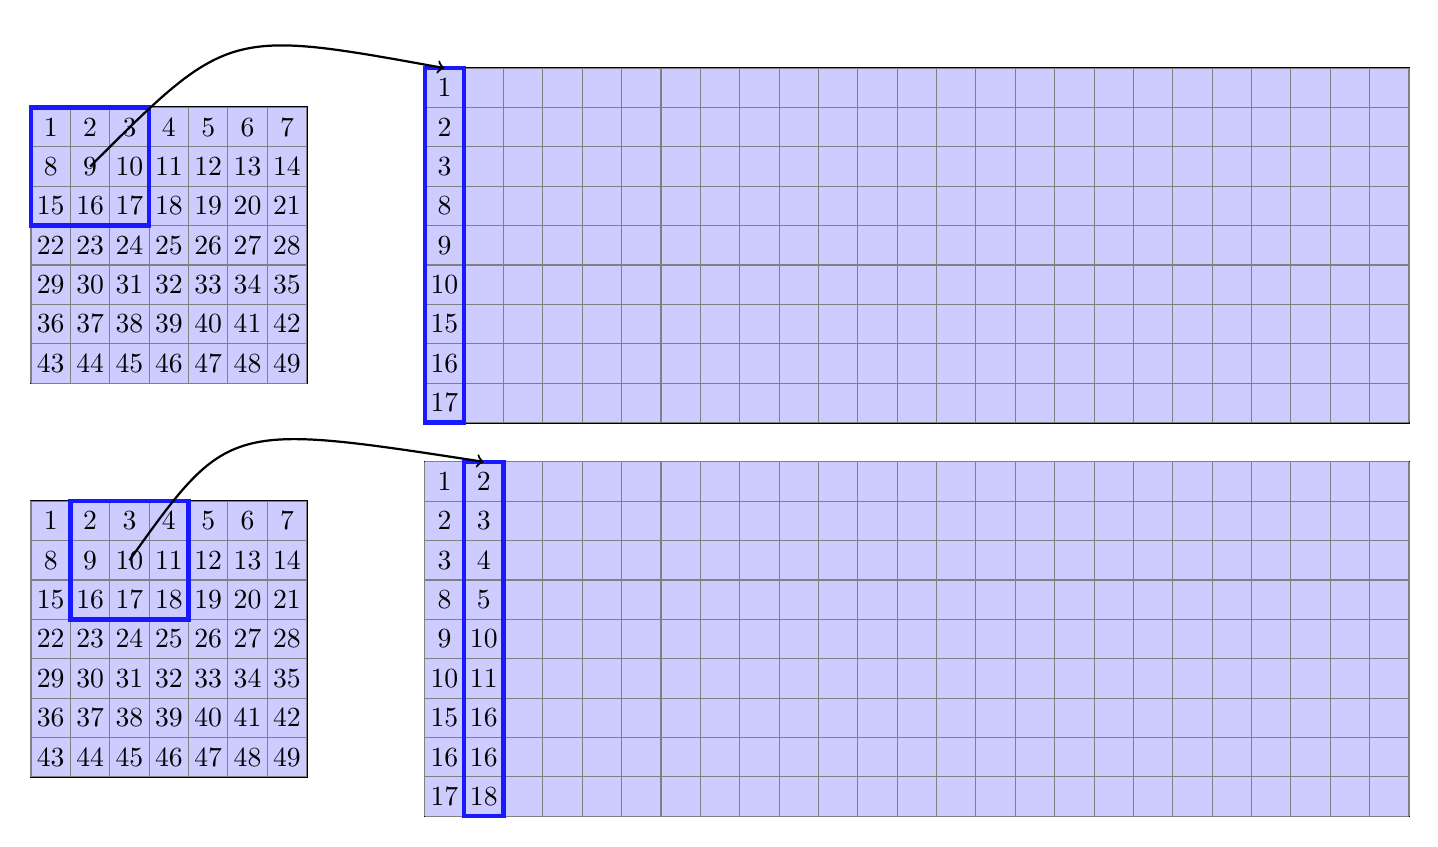
\begin{tikzpicture}
        \begin{scope}[scale=0.5]
            % draw input convolution
            % draw outer rectangle border
            \draw[thick] (0,0) rectangle (7,7);
            
            % Fill the entire 7x7 grid area with a light blue color
            \fill[blue!20] (0,0) rectangle (7,7);
       
            % Draw the boundary of each grid
            \draw[step=1cm, gray, thin] (0,0) grid (7,7); 

            % Draw kernel convolution
            % Draw the outer rectangle border
            \draw[ultra thick,blue!90] (0,4) rectangle (3,7);

            % fill the number in grid
            \foreach \row in{0,...,6}{
                \foreach \col in {0,...,6}{
                    \node at (\col+0.5,6.5-\row){\pgfmathparse{int(\row*7+\col+1)}\pgfmathresult};
                }
            }



            % draw the output of im2col

            \draw[thick] (10,8) rectangle (35,-1);
            
            % Fill the entire 7x7 grid area with a light blue color
            \fill[blue!20] (10,8) rectangle (35,-1);
       
            % Draw the boundary of each grid
            \draw[step=1cm, gray, thin] (10,8) grid (35,-1); 
            \draw[ultra thick,blue!90] (10,8) rectangle (11,-1);
            % fill the flatten values in sliding window manually
            \node at (10.5,7.5) {1};
            \node at (10.5,6.5) {2};
            \node at (10.5,5.5) {3};
            \node at (10.5,4.5) {8};
            \node at (10.5,3.5) {9};
            \node at (10.5,2.5) {10};
            \node at (10.5,1.5) {15};
            \node at (10.5,0.5) {16};
            \node at (10.5,-0.5) {17};

            % draw arrow from im to col
            \draw[->,thick] (1.5,5.5) .. controls (5,9) .. (10.5,8);

        \end{scope}


        \begin{scope}[scale=0.5,yshift=-10cm]
            % draw input convolution
            % draw outer rectangle border
            \draw[thick] (0,0) rectangle (7,7);
            
            % Fill the entire 7x7 grid area with a light blue color
            \fill[blue!20] (0,0) rectangle (7,7);
       
            % Draw the boundary of each grid
            \draw[step=1cm, gray, thin] (0,0) grid (7,7); 

            % Draw kernel convolution
            % Draw the outer rectangle border
            \draw[ultra thick,blue!90] (1,4) rectangle (4,7);

            % fill the number in grid
            \foreach \row in{0,...,6}{
                \foreach \col in {0,...,6}{
                    \node at (\col+0.5,6.5-\row){\pgfmathparse{int(\row*7+\col+1)}\pgfmathresult};
                }
            }



            % draw the output of im2col

            \draw[thick] (10,8) rectangle (35,-1);
            
            % Fill the entire 7x7 grid area with a light blue color
            \fill[blue!20] (10,8) rectangle (35,-1);
       
            % Draw the boundary of each grid
            \draw[step=1cm, gray, thin] (10,8) grid (35,-1); 

            \draw[ultra thick,blue!90] (11,8) rectangle (12,-1);
            % fill the flatten values in sliding window manually
            \node at (10.5,7.5) {1};
            \node at (10.5,6.5) {2};
            \node at (10.5,5.5) {3};
            \node at (10.5,4.5) {8};
            \node at (10.5,3.5) {9};
            \node at (10.5,2.5) {10};
            \node at (10.5,1.5) {15};
            \node at (10.5,0.5) {16};
            \node at (10.5,-0.5) {17};


            \node at (11.5,7.5) {2};
            \node at (11.5,6.5) {3};
            \node at (11.5,5.5) {4};
            \node at (11.5,4.5) {5};
            \node at (11.5,3.5) {10};
            \node at (11.5,2.5) {11};
            \node at (11.5,1.5) {16};
            \node at (11.5,0.5) {16};
            \node at (11.5,-0.5) {18};

            % draw arrow from im to col
            \draw[->,thick] (2.5,5.5) .. controls (5,9) .. (11.5,8);

        \end{scope}
    \end{tikzpicture}
    \centering
    \caption{Step1: Image to Column (Im2Col) operation is to sort all values in convolutional kernel in a column}
    \label{fig:im2col}
\end{figure}



\begin{figure}[H]
    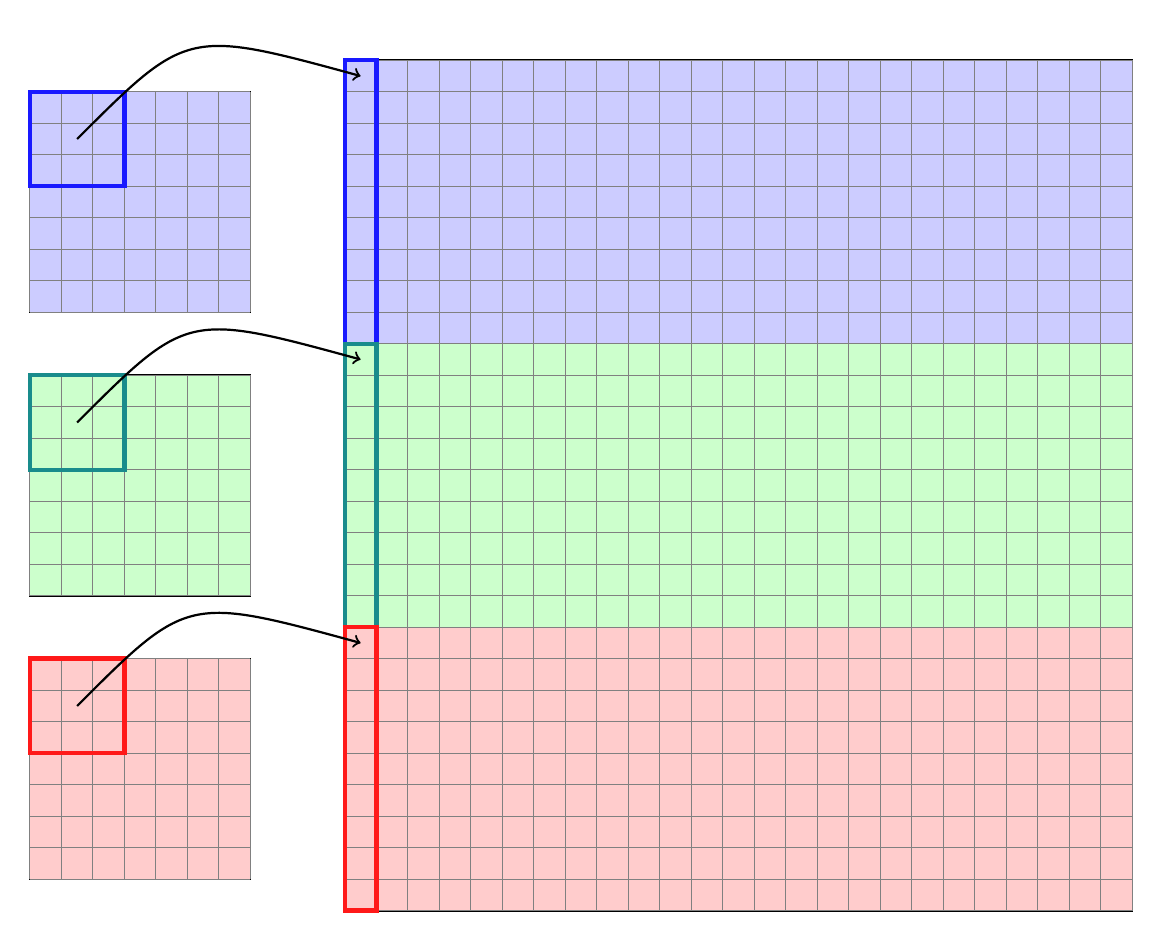
\begin{tikzpicture}
        \begin{scope}[scale=0.4]
            % 3 channels rectangular input
            \draw[thick] (0,0) rectangle (7,7);
            \draw[thick] (0,-9) rectangle (7,-2);
            \draw[thick] (0,-18) rectangle (7,-11);
            % Fill the entire 7x7 grid area with a light blue color
            \fill[blue!20] (0,0) rectangle (7,7);
            \fill[green!20] (0,-9) rectangle (7,-2);
            \fill[red!20] (0,-18) rectangle (7,-11);
       
            % Draw the boundary of each grid
            \draw[step=1cm, gray, thin] (0,0) grid (7,7); 
            \draw[step=1cm, gray, thin] (0,-9) grid (7,-2); 
            \draw[step=1cm, gray, thin] (0,-18) grid (7,-11); 

            
            % Draw the outer rectangle border
            \draw[ultra thick,blue!90] (0,4) rectangle (3,7);
            \draw[ultra thick,teal!90] (0,-5) rectangle (3,-2);
            \draw[ultra thick,red!90] (0,-14) rectangle (3,-11);



            % draw the output of im2col
            \draw[thick] (10,8) rectangle (35,-19);
            % fill the column for each component matrix corresponding to channel dim
            \fill[blue!20] (10,8) rectangle (35,-1);
            \fill[green!20] (10,-1) rectangle (35,-10);
            \fill[red!20] (10,-10) rectangle (35,-19);
       
            % Draw the boundary of each grid
            \draw[step=1cm, gray, thin] (10,8) grid (35,-19); 
            
            \draw[ultra thick,blue!90] (10,8) rectangle (11,-1);
            \draw[ultra thick,teal!90] (10,-1) rectangle (11,-10);
            \draw[ultra thick,red!90] (10,-10) rectangle (11,-19);


            % draw arrow from im to col
            \draw[->,thick] (1.5,5.5) .. controls (5,9) .. (10.5,7.5);
            \draw[->,thick] (1.5,-3.5) .. controls (5,0) .. (10.5,-1.5);
            \draw[->,thick] (1.5,-12.5) .. controls (5,-9) .. (10.5,-10.5);
        \end{scope}
    \end{tikzpicture}
    \centering
    \caption{The output Im2col in 3-channels image}
\end{figure}


\begin{figure}[H]
    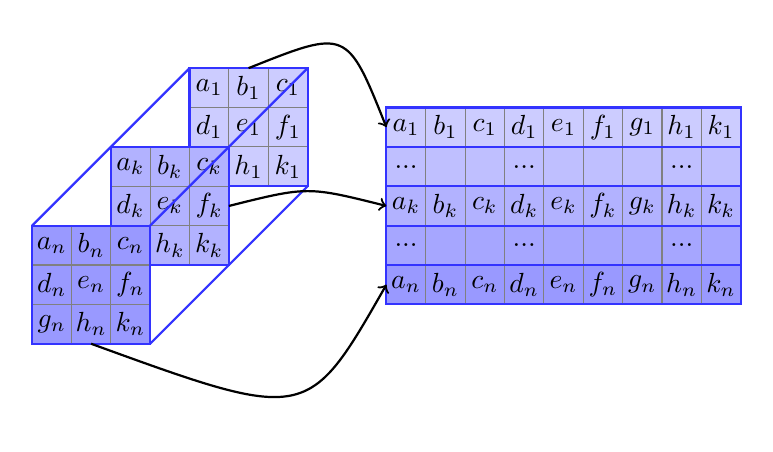
\begin{tikzpicture}
        \begin{scope}[scale=0.5]
            % Draw the outer rectangle border
            \fill[blue!20] (0,0) rectangle (3,3);
            \draw[step=1cm, gray, thin] (0,0) grid (3,3); 
            \draw[thick,blue!80] (0,0) rectangle (3,3);
            
            \fill[blue!30] (-2,-2) rectangle (1,1);
            \draw[step=1cm, gray, thin] (-2,-2) grid (1,1); 
            \draw[thick,blue!80] (-2,-2) rectangle (1,1);

            \fill[blue!40] (-4,-4) rectangle (-1,-1);
            \draw[step=1cm, gray, thin] (-4,-4) grid (-1,-1); 
            \draw[thick,blue!80] (-4,-4) rectangle (-1,-1);

            
            
            \node at (0.5,2.5) {$a_{1}$};
            \node at (1.5,2.5) {$b_{1}$};
            \node at (2.5,2.5) {$c_{1}$};
            \node at (0.5,1.5) {$d_{1}$};
            \node at (1.5,1.5) {$e_{1}$};
            \node at (2.5,1.5) {$f_{1}$};
            %\node at (0.5,0.5) {g};
            \node at (1.5,0.5) {$h_{1}$};
            \node at (2.5,0.5) {$k_{1}$};

            \node at (-1.5,0.5) {$a_{k}$};
            \node at (-0.5,0.5) {$b_{k}$};
            \node at (0.5,0.5) {$c_{k}$};
            \node at (-1.5,-0.5) {$d_{k}$};
            \node at (-0.5,-0.5) {$e_{k}$};
            \node at (0.5,-0.5) {$f_{k}$};
            %\node at (-1.5,-1.5) {g};
            \node at (-0.5,-1.5) {$h_{k}$};
            \node at (0.5,-1.5) {$k_{k}$};
           
            \node at (-3.5,-1.5) {$a_{n}$};
            \node at (-2.5,-1.5) {$b_{n}$};
            \node at (-1.5,-1.5) {$c_{n}$};
            \node at (-3.5,-2.5) {$d_{n}$};
            \node at (-2.5,-2.5) {$e_{n}$};
            \node at (-1.5,-2.5) {$f_{n}$};
            \node at (-3.5,-3.5) {$g_{n}$};
            \node at (-2.5,-3.5) {$h_{n}$};
            \node at (-1.5,-3.5) {$k_{n}$};
           
            \draw[thick,blue!80] (-4,-1) -- (0,3);
           \draw[thick,blue!80] (-1,-1) -- (3,3); 
           \draw[thick,blue!80] (-1,-4) -- (3,0);
            
            \fill[blue!20] (5,1) rectangle (14,2);
            \draw[step=1cm, gray, thin] (5,1) grid (14,2);
           \draw[thick,blue!80] (5,1) rectangle (14,2);
           
            \fill[blue!25] (5,0) rectangle (14,1);
            \draw[step=1cm, gray, thin] (5,0) grid (14,1);
            \draw[thick,blue!80] (5,0) rectangle (14,1);
            
            \fill[blue!30] (5,-1) rectangle (14,0);
            \draw[step=1cm, gray, thin] (5,-1) grid (14,0);
            \draw[thick,blue!80] (5,-1) rectangle (14,0);
            
            \fill[blue!35] (5,-2) rectangle (14,-1);
            \draw[step=1cm, gray, thin] (5,-2) grid (14,-1);
            \draw[thick,blue!80] (5,-2) rectangle (14,-1);
            
            \fill[blue!40] (5,-3) rectangle (14,-2);
            \draw[step=1cm, gray, thin] (5,-3) grid (14,-2);
            \draw[thick,blue!80] (5,-3) rectangle (14,-2);

            \node at (5.5,1.5) {$a_{1}$};
            \node at (6.5,1.5) {$b_{1}$};
            \node at (7.5,1.5) {$c_{1}$};
            \node at (8.5,1.5) {$d_{1}$};
            \node at (9.5,1.5) {$e_{1}$};
            \node at (10.5,1.5){$f_{1}$};
            \node at (11.5,1.5) {$g_{1}$};
            \node at (12.5,1.5){$h_{1}$};
            \node at (13.5,1.5){$k_{1}$};


            \node at (5.5,0.5) {...};
            \node at (8.5,0.5) {...};
            \node at (12.5,0.5) {...};



            \node at (5.5,-0.5) {$a_{k}$};
            \node at (6.5,-0.5) {$b_{k}$};
            \node at (7.5,-0.5) {$c_{k}$};
            \node at (8.5,-0.5) {$d_{k}$};
            \node at (9.5,-0.5) {$e_{k}$};
            \node at (10.5,-0.5){$f_{k}$};
            \node at (11.5,-0.5) {$g_{k}$};
            \node at (12.5,-0.5){$h_{k}$};
            \node at (13.5,-0.5){$k_{k}$};

            \node at (5.5,-1.5) {...};
            \node at (8.5,-1.5) {...};
            \node at (12.5,-1.5) {...};
            
            \node at (5.5,-2.5) {$a_{n}$};
            \node at (6.5,-2.5) {$b_{n}$};
            \node at (7.5,-2.5) {$c_{n}$};
            \node at (8.5,-2.5) {$d_{n}$};
            \node at (9.5,-2.5) {$e_{n}$};
            \node at (10.5,-2.5){$f_{n}$};
            \node at (11.5,-2.5) {$g_{n}$};
            \node at (12.5,-2.5){$h_{n}$};
            \node at (13.5,-2.5){$k_{n}$};

            % draw arrow
            \draw[->,thick] (1.5,3) .. controls (4,4) .. (5,1.5);
            \draw[->,thick] (1,-0.5) .. controls (3,0) .. (5,-0.5);
            \draw[->,thick] (-2.5,-4) .. controls (3,-6) .. (5,-2.5);
        \end{scope}
    \end{tikzpicture}
    \centering
    \caption{Reshape the kernel to row vector form. Given there are N kernels, then the reshaped kernels set will have the concatenated row vectors}
    \label{fig:reshaped_kernels}
\end{figure}


\begin{figure}[H]
    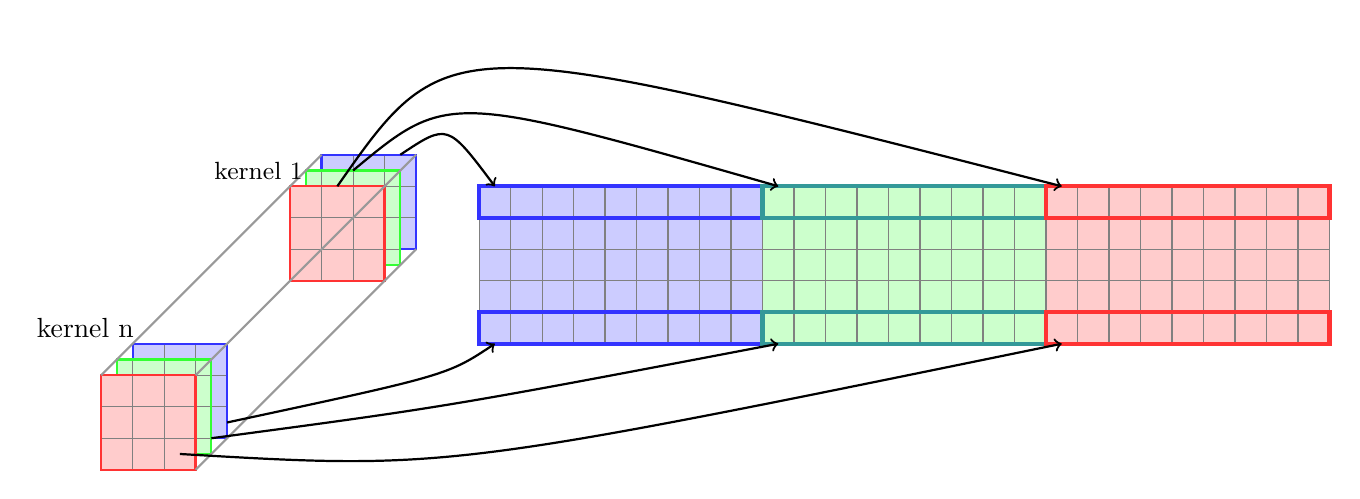
\begin{tikzpicture}
        \begin{scope}[scale=0.4]
            % set of kernel 1
            \fill[blue!20] (0,0) rectangle (3,3);
            \draw[step=1cm, gray, thin] (0,0) grid (3,3); 
            \draw[thick,blue!80] (0,0) rectangle (3,3);

            \fill[green!20] (-0.5,-0.5) rectangle (2.5,2.5);
            \draw[step=1cm, gray, thin] (-0.5,-0.5) grid (2.5,2.5); 
            \draw[thick,green!80] (-0.5,-0.5) rectangle (2.5,2.5);

            \fill[red!20] (-1,-1) rectangle (2,2);
            \draw[step=1cm, gray, thin] (-1,-1) grid (2,2); 
            \draw[thick,red!80] (-1,-1) rectangle (2,2);

            % set of kernel n            
            \fill[blue!20] (-6,-6) rectangle (-3,-3);
            \draw[step=1cm, gray, thin] (-6,-6) grid (-3,-3); 
            \draw[thick,blue!80] (-6,-6) rectangle (-3,-3);

            \fill[green!20] (-6.5,-6.5) rectangle (-3.5,-3.5);
            \draw[step=1cm, gray, thin] (-6.5,-6.5) grid (-3.5,-3.5); 
            \draw[thick,green!80] (-6.5,-6.5) rectangle (-3.5,-3.5);

            \fill[red!20] (-7,-7) rectangle (-4,-4);
            \draw[step=1cm, gray, thin] (-7,-7) grid (-4,-4); 
            \draw[thick,red!80] (-7,-7) rectangle (-4,-4);

            % line represent the set of kernels
            \draw[thick,gray!80] (-7,-4) -- (0,3);
           \draw[thick,gray!80] (-4,-4) -- (3,3); 
           \draw[thick,gray!80] (-4,-7) -- (3,0);

            
           % denote the kernels
           \node at (-2,2.5) {\small{kernel 1}};
           \node at (-7.5,-2.5) {kernel n};


           
           % reshape kernels
            \fill[blue!20] (5,-3) rectangle (14,2);
            \draw[step=1cm, gray, thin] (5,-3) grid (14,2);
           \draw[ultra thick,blue!80] (5,-3) rectangle (14,-2);
           \draw[ultra thick,blue!80] (5,1) rectangle (14,2);
           
            \fill[green!20] (14,-3) rectangle (23,2);
            \draw[step=1cm, gray, thin] (14,-3) grid (23,2);
           \draw[ultra thick,teal!80] (14,-3) rectangle (23,-2);
           \draw[ultra thick,teal!80] (14,1) rectangle (23,2);
           

            \fill[red!20] (23,-3) rectangle (32,2);
            \draw[step=1cm, gray, thin] (23,-3) grid (32,2);
           \draw[ultra thick,red!80] (23,-3) rectangle (32,-2);
           \draw[ultra thick,red!80] (23,1) rectangle (32,2);
           

            % draw arrow
           \draw[->,thick] (2.5,3) .. controls (4,4) .. (5.5,2);
            \draw[->,thick] (1,2.5) .. controls (4,5) .. (14.5,2);
            \draw[->,thick] (0.5,2) .. controls (4,7) .. (23.5,2);
           
            \draw[->,thick] (-3,-5.5) .. controls (4,-4) .. (5.5,-3);
            \draw[->,thick] (-3.5,-6) .. controls (4,-5) .. (14.5,-3);
            \draw[->,thick] (-4.5,-6.5) .. controls (4,-7) .. (23.5,-3);

            % ex
        \end{scope}
    \end{tikzpicture}
    \centering
    \caption{Reshape kernel in 3-channels }
    \label{fig:reshaped_kernels_3_channels}
\end{figure}




\begin{figure}[H]
    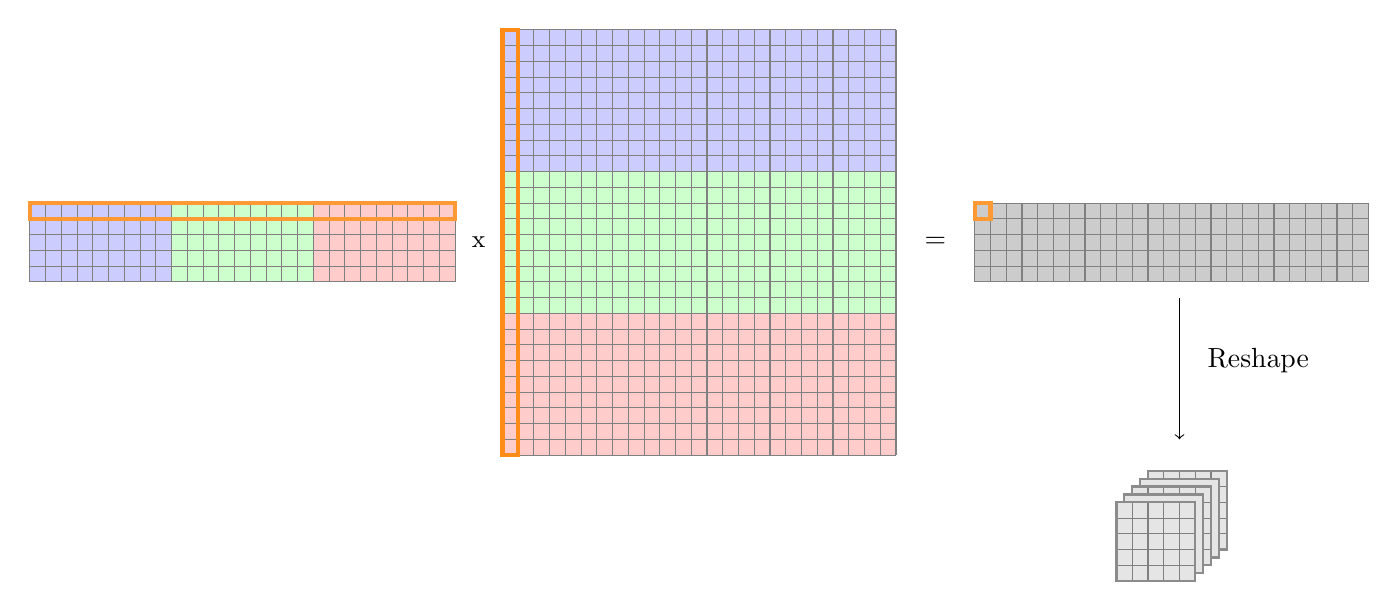
\begin{tikzpicture}
        \begin{scope}[scale=0.2]
            % ouput Im2Col            
            \fill[blue!20] (35,8) rectangle (60,-1);
            \fill[green!20] (35,-1) rectangle (60,-10);
            \fill[red!20] (35,-10) rectangle (60,-19);
            \draw[step=1cm, gray, thin] (35,8) grid (60,-19); 
            \draw[ultra thick,orange!90] (35,8) rectangle (36,-19);

            \node at (33.5,-5.5) {\small{x}};

            % Reshaped kernels
            \fill[blue!20] (5,-8) rectangle (14,-3);
            \draw[step=1cm, gray, thin] (5,-8) grid (14,-3);
           
            \fill[green!20] (14,-8) rectangle (23,-3);
            \draw[step=1cm, gray, thin] (14,-8) grid (23,-3);
           

            \fill[red!20] (23,-8) rectangle (32,-3);
            \draw[step=1cm, gray, thin] (23,-8) grid (32,-3);
           \draw[ultra thick,orange!80] (5,-4) rectangle (32,-3); 
        
           \node at (62.5,-5.5) {=};
            % output matrix multiplication
            \fill[gray!40] (65,-8) rectangle (90,-3);
            \draw[step=1cm, gray, thin] (65,-8) grid (90,-3); 
            \draw[ultra thick, orange!80] (65,-4) rectangle (66,-3);

            \draw[->] (78,-9) -- (78,-18);
            \node at (83,-13) {Reshape};
           
            % reshape form
            \fill[gray!20] (76,-25) rectangle (81,-20);
            \draw[step=1cm, gray, thin] (76,-25) grid (81,-20);
            \draw[thick,gray!90] (76,-25) rectangle (81,-20);

            \fill[gray!20] (75.5,-25.5) rectangle (80.5,-20.5);
            %\draw[step=1cm, gray, thin] (75.5,-25.5) grid (80.5,-20.5);
            \draw[thick,gray!90] (75.5,-25.5) rectangle (80.5,-20.5);
        
            \fill[gray!20] (75,-26) rectangle (80,-21);
            \draw[step=1cm, gray, thin] (75,-26) grid (80,-21);
            \draw[thick,gray!90] (75,-26) rectangle (80,-21);

            \fill[gray!20] (74.5,-26.5) rectangle (79.5,-21.5);
            %\draw[step=1cm, gray, thin] (74.5,-26.5) grid (79.5,-21.5);
            \draw[thick,gray!90] (74.5,-26.5) rectangle (79.5,-21.5);

            \fill[gray!20] (74,-27) rectangle (79,-22);
            \draw[step=1cm, gray, thin] (74,-27) grid (79,-22);
            \draw[thick,gray!90] (74,-27) rectangle (79,-22);

        \end{scope}
    \end{tikzpicture}
    \centering
    \caption{Matrix multiplication operation between reshaped kernels and Im2Col output. The output of this operation will be reshaped to the expected form as the same as after convolution.}
    \label{fig:matrix_multiplication}
\end{figure}
